\documentclass[tikz,border={0 1}]{standalone}
% \usepackage{dejavu}
\usepackage[scaled=0.9]{DejaVuSansMono}
% \usepackage{stackrel}

\usetikzlibrary{patterns,decorations.markings,backgrounds}
\usetikzlibrary{decorations.pathreplacing}

\begin{document}
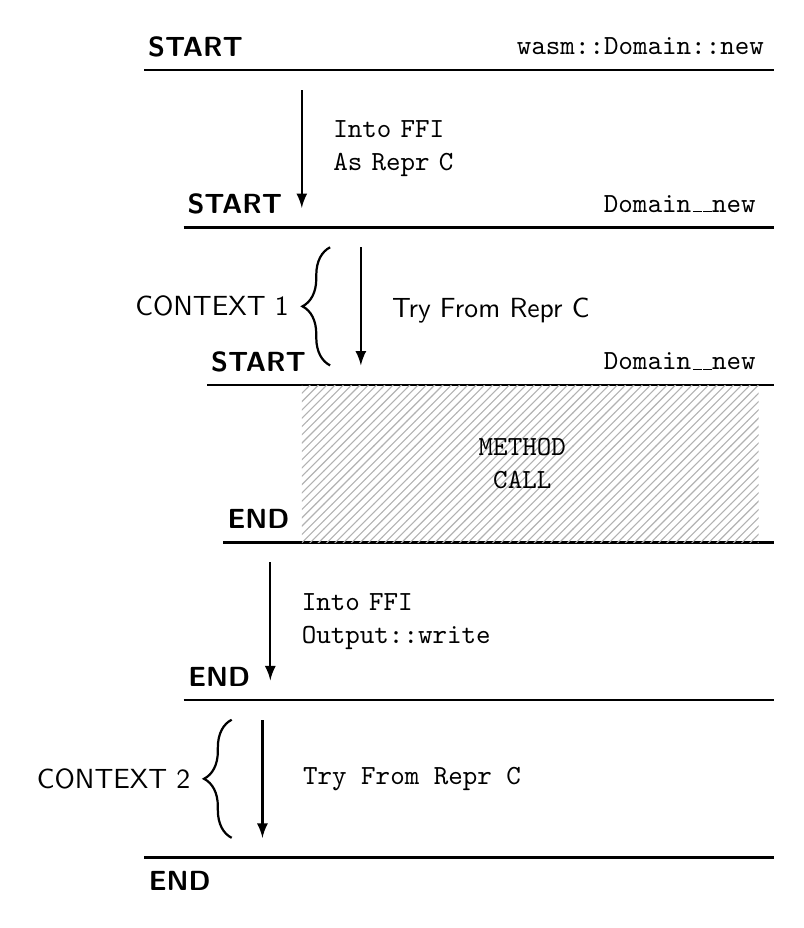
\begin{tikzpicture}[thick]


\coordinate (A_l) at (0, 0);  \coordinate (A_r) at (8, 0);
\coordinate (B_l) at (0.5, 2);  \coordinate (B_r) at (8, 2);
\coordinate (C_l) at (1, 4);  \coordinate (C_r) at (8, 4);
\coordinate (D_l) at (0.8, 6);  \coordinate (D_r) at (8, 6);
\coordinate (E_l) at (0.5, 8);  \coordinate (E_r) at (8, 8);
\coordinate (F_l) at (0, 10); \coordinate (F_r) at (8, 10);


\node[shift={(0.65,0.3)}, font=\sffamily\bfseries] at (F_l) {START};
\node[shift={(0.65,0.3)}, font=\sffamily\bfseries] at (E_l) {START};
\node[shift={(0.65,0.3)}, font=\sffamily\bfseries] at (D_l) {START};

\node[shift={(0.45,-0.3)}, font=\sffamily\bfseries] at (A_l) {END};
\node[shift={(0.45,0.3)}, font=\sffamily\bfseries] at (B_l)  {END};
\node[shift={(0.45,0.3)}, font=\sffamily\bfseries] at (C_l)  {END};

\node[shift={(-1.7,0.3)}, font=\sffamily] at (F_r) {\texttt{wasm::Domain::new}};
\node[shift={(-1.2,0.3)}, font=\sffamily] at (E_r) {\texttt{Domain\_\_new}};
\node[shift={(-1.2,0.3)}, font=\sffamily] at (D_r) {\texttt{Domain\_\_new}};

\draw (A_l) -- (A_r);
\draw (B_l) -- (B_r);
\draw (C_l) -- (C_r);
\draw (D_l) -- (D_r);
\draw (E_l) -- (E_r);
\draw (F_l) -- (F_r);

% Top arrow
\draw [latex-](2.,8.25) -- (2.,9.75);
% 2nd top arrow
\draw [latex-](2.75,6.25) -- (2.75,7.75);
\draw [decorate,decoration={brace,amplitude=10pt},xshift=-4pt,yshift=0pt]
(2.5,6.25) -- (2.5,7.75) node [black,midway,xshift=-1.5cm, font=\sffamily] 
{CONTEXT 1};
% 3rd top arrow
\draw [latex-](1.6,2.25) -- (1.6,3.75);
% 4rd top arrow
\draw [latex-](1.5,0.25) -- (1.5,1.75);
% 4rd brace
\draw [decorate,decoration={brace,amplitude=10pt},xshift=-4pt,yshift=0pt]
(1.25,0.25) -- (1.25,1.75) node [black,midway,xshift=-1.5cm, font=\sffamily]
{CONTEXT 2};

\definecolor{grey}{rgb}{0.7,0.7,0.7}
\path[
    pattern=north east lines,
    pattern color=grey
] (2,4) rectangle (7.8,6);

\node[text width=2cm, font=\sffamily] at (3.4,9.0) {\texttt{Into FFI \\ As Repr C}};

\node[font=\sffamily] at (4.4,6.95) {Try From Repr C};

\node[text width=3cm, text centered, font=\sffamily\bfseries] at (4.8,5.0) {\texttt{METHOD \\ CALL}};

\node[text width=2cm, font=\sffamily] at (3.0,3.0) {\texttt{Into FFI \\ Output::write}};

\node[font=\sffamily] at (3.4,1) {\texttt{Try From Repr C}};

\end{tikzpicture}
\end{document}
